%%%%%%%%%%%%%%%%%%%%%%%%%%%%%%%%%%%%%%%%%%%%%%%%%%%%%%%%%%%%%%%%%%%%%%%%
%                                                                      %
%     File: Thesis_Implementation.tex                                  %
%     Tex Master: Thesis.tex                                           %
%                                                                      %
%     Author: Andre C. Marta                                           %
%     Last modified :  2 Jul 2015                                      %
%                                                                      %
%%%%%%%%%%%%%%%%%%%%%%%%%%%%%%%%%%%%%%%%%%%%%%%%%%%%%%%%%%%%%%%%%%%%%%%%

\chapter{Algorithm}
\label{chapter:algorithm}

Our algorithm is performed in eight steps (see Figure~\ref{fig:crsh}). In each frame steps 1 and 2 are executed just once while steps 3 through 6 are executed once per ray batch. Batches can consist of any combination of shadow rays, reflection rays or refraction rays.

\begin{figure}[!htb]
    \centering
    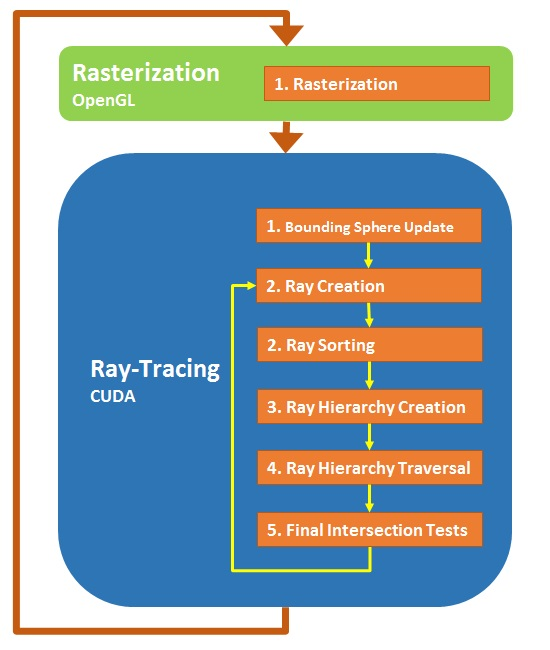
\includegraphics[width=0.45\textwidth]{Images/Overview}
    \caption{\label{fig:crsh}Coherent Ray-Space Hierarchy Overview.}
\end{figure}

%%%%%%%%%%%%%%%%%%%%%%%%%%%%%%%%%%%%%%%%%%%%%%%%%%%%%%%%%%%%%%%%%%%%%%%%
\section{Rasterization}
\label{section:algorithm-rasterization}

Rasterization is performed as a first step. There was in the path an ongoing urban legend that Rasterization and Ray-Tracing are polar opposites and that a choice has to be made between these two techniques. This is not true at all. Although Rasterization solves the rendering problem conversely vs Ray-Tracing (i.e. projecting primitives to the screen, vs projecting rays backwards to the primitives in the scene), one can complement the other. The first set of rays, the primary rays, does not convey any of the global illumination effects that Ray-Tracing is well suited to achieve, such as Shadows, Reflections and Refractions. This means that Rasterization can convey similar visual results to tracing the primary rays, while being extremely faster and optimized in the graphics hardware. Supplementing the Rasterization of primary rays with the Ray-Tracing of secondary rays can get us the benefits from both techniques: the efficiency of Rasterization and the global illumination effects from Ray-Tracing.

\medskip

In order to combine both techniques the output from the fragment shaders used to rasterize the scene must be more than just the traditional fragment colors. We need to create different render targets according to the information we want to store. In our case we output the fragment diffuse and specular properties, the fragment position and the fragment normal. In our implementation the fragment shader outputs 4 different textures containing four 32 bit floats per pixel each. These textures are generated with OpenGL/GLSL and are then sent to CUDA to create the first level of secondary rays.

%%%%%%%%%%%%%%%%%%%%%%%%%%%%%%%%%%%%%%%%%%%%%%%%%%%%%%%%%%%%%%%%%%%%%%%%
\section{Ray-Tracing}
\label{section:algorithm-ray-tracing}

\subsection{Bounding Volume Update}
Here we update the object bounding spheres according to the transformations being applied to the object they contain (e.g. translation, scale). Since we only update the center and the radius there is no need to recalculate the bounding spheres in each frame (transformations do not invalidate the bounding spheres).

We pre-compute the minimum bounding sphere of the object meshes, using an implementation based on \cite{Gartner99}s algorithm, so there is no impact on render time performance for this computation.

\subsection{Secondary Ray Generation and Indexing}

After the Rasterization step we need to generate the secondary rays. We create an index for each individual ray in order to speed up ray sorting in the following steps. We use a different hashing function for each type of ray (see Figures~\ref{fig:sr}, ~\ref{fig:rr}). Since each ray consists of an origin and a direction it would be straightforward to use these two parameters to create our hash. However for shadow rays it is sufficient to use the light-index, to which it belongs, and the ray direction. This is doable if we invert the origin of the shadow ray so that it is located at the light source rather than the originating fragment. To further reduce the size of the hash keys we convert the ray direction into spherical coordinates \cite{GraphicGems5} and store both the light index and the spherical coordinates into a 32 bit integer, with the light index having the higher bit-value such that the shadow rays are sorted according to the light source a priori.

\begin{figure}[!htb]
    \centering
    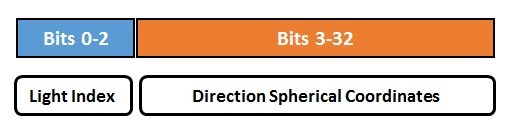
\includegraphics[scale=0.75]{Images/Shadow_Hash}
    \caption{\label{fig:sr}Shadow Ray Hash.}
\end{figure}

The Reflection and Refraction rays are also converted to spherical coordinates. However in this case the ray origin is used in the hash, given that these rays are not coherent with regards to the origin, unlike shadow rays.

\begin{figure}[!htb]
    \centering
    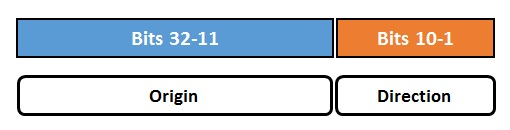
\includegraphics[scale=0.75]{Images/Reflection_Hash}
    \caption{\label{fig:rr}Reflection and Refraction Ray Hash.}
\end{figure}

Once generation is complete, we have an array with the generated secondary rays as well as two arrays with the ray keys (ray hashes) and the ray values (ray position in the ray array) and a final array with head flags which indicate if there is a ray in the corresponding position within the key-value arrays, where we store either a 0 or a 1, indicating if there is a ray or not, respectively.
Using the information from the head flags array we then run a trimming operator on the key-value arrays (see Figure~\ref{fig:at}). This is done by first applying an inclusive scan operator \cite{Merrill09} on the head flags array, which gives us the number of positions each pair needs to be shifted to the left. This is done in order to trim the arrays \cite{GPUGems2}.

\begin{figure}[!htb]
    \centering
    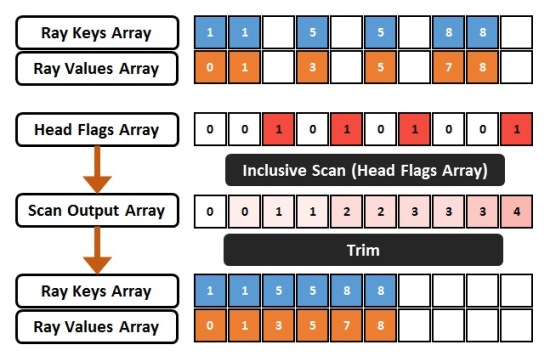
\includegraphics[scale=0.75]{Images/Array_Trimming}
    \caption{\label{fig:at}Array Trimming}
\end{figure}

\subsection{Secondary Ray Compression}

Here we use a compression-sorting-decompression scheme, expanding on prior work by Garanzha and Loops \cite{Garanzha10}. The compression step exploits the local coherency of rays. Even for secondary rays, the bounces generated by two adjacent rays have a good chance of being coherent. This can result in the same hash value for both bounces. Given this information, we compress the ray key-value pairs into chunks, minimizing the number of pairs that need to be sorted. To compress the pairs we utilize a head flags array with the same size as the key-value pair array, initializing it with $0$s in every position and inserting $1$s into positions in which the key (hash) of the corresponding pair differs from the previous pair. After populating the head flags array we apply an inclusive scan operator on it \cite{Merrill09}. By combining the head flags array with the scan output array we create the chunk keys, base and size arrays, which contain the hash, starting index and size of the corresponding chunks (see Figure~\ref{fig:rcc}). The chunk keys are represented in different colors at the image below. The chunk base array represents the original position of the first ray in the chunk while the chunk size array represents the size of the chunk, needed for the ray array decompression.

\begin{figure}[!htb]
    \centering
    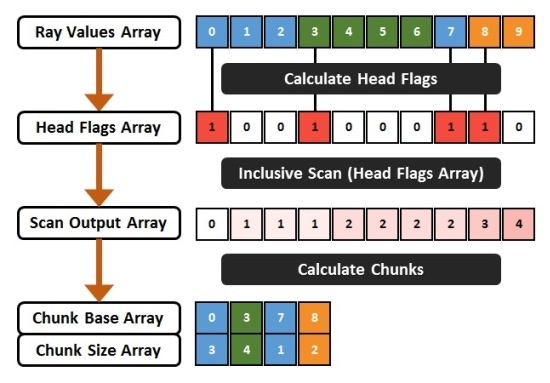
\includegraphics[scale=0.75]{Images/Ray_Compression}
    \caption{\label{fig:rcc}Ray Compression into Chunks}
\end{figure}

\subsection{Secondary Ray Sorting}

After ray compression we have an array of chunks with the information required to reconstruct the initial rays array. So we can begin the actual sorting. We radix sort \cite{Merrill11} the chunks array according to the chunk keys.

\subsection{Secondary Ray Decompression}

Decompression works by creating a skeleton array. This skeleton array is similar to the head flag arrays we created before except that it contains the size of the sorted chunks. Next we apply an exclusive scan operator on the skeleton array. This will give us the positions of the chunks starting positions on the sorted key and value arrays. After creating these two arrays for each position in the scan array we fill the sorted ray array. We start in the position indicated in the scan array and finish after filling the number of rays contained within the corresponding chunk.

\begin{figure}[!htb]
    \centering
    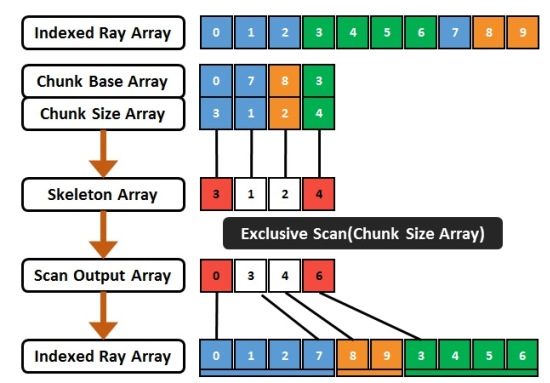
\includegraphics[scale=0.75]{Images/Ray_Decompression}
    \caption{Ray Decompression from Chunks}
\end{figure}

\subsection{Hierarchy Creation}

With the sorted rays we can now create the actual hierarchy. Since the rays are now sorted coherently the hierarchy will be much tighter in its lower levels, giving us a smaller number of intersection candidates as we traverse further down the hierarchy.
Each node in the hierarchy is represented by a sphere and a cone (see Figures~\ref{fig:bc}, \ref{fig:bs}).

\begin{figure}[!htb]
    \centering
    
    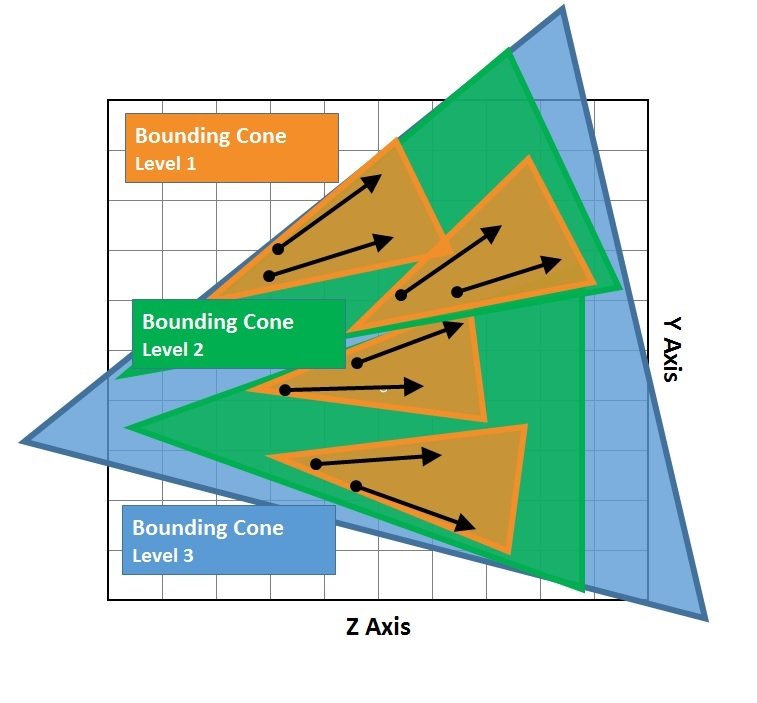
\includegraphics[scale=0.30]{Images/Bounding_Cone}
    \caption{\label{fig:bc}Bounding Cone - 2D View}

    \vspace{2.5pt}

    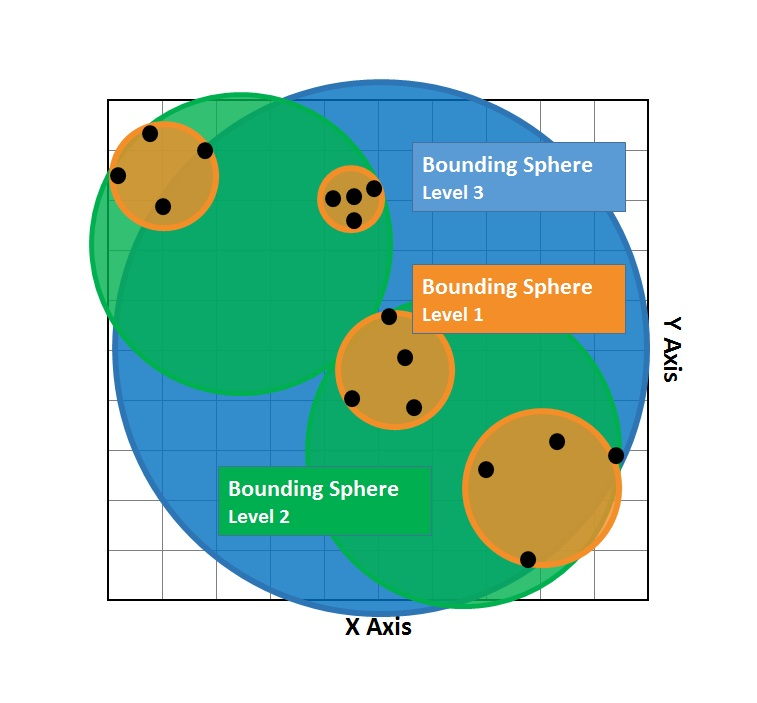
\includegraphics[scale=0.30]{Images/Bounding_Sphere}
    \caption{\label{fig:bs}Bounding Sphere - 2D View}
\end{figure}

The sphere contains all the nodes ray origins while the cone contain the rays themselves (see Figure~\ref{fig:cru}). This structure is stored using eight floats: the sphere center and radius (four floats) and the cone direction and spread angle (four floats). The construction of the hierarchy is done in a bottom-up fashion. Thus we start with the leaves, with spheres of radius $0$ and a cone with spread angle equal to $0$. These leaves correspond to the sorted rays. The upper levels of the hierarchy are created by calculating the union of the child nodes. The number of children combined in each node can also be parametrized. 

\begin{figure}[!htb]
    \centering
    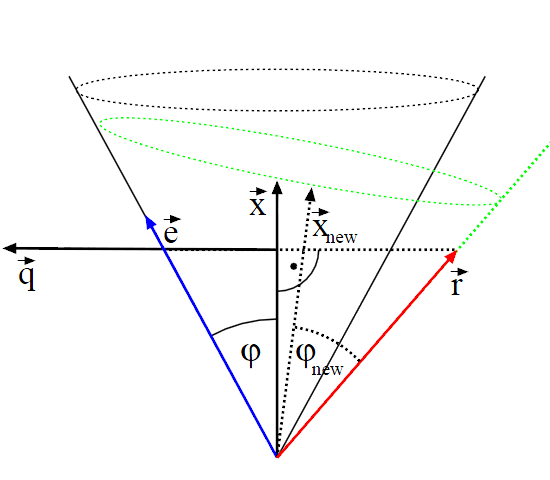
\includegraphics[scale=0.30]{Images/Cone_Union}
    \caption{\label{fig:cru}Cone-Ray Union - 2D View. \small{courtesy of \cite{Szecsi06}}.}
\end{figure}

For the first level of nodes we use the formulas below to create compact cones \cite{Szecsi06}.

\begin{equation}
    \vec{q} = \frac{ (\vec{x} \cdot \vec{r}) \cdot \vec{x} - \vec{r} }
                   {|(\vec{x} \cdot \vec{r}) \cdot \vec{x} - \vec{r}|}
\end{equation}

\begin{equation}
    \vec{e} = \vec{x} \cdot \cos(\phi) + \vec{q} \cdot \sin{\phi}
\end{equation}

\begin{equation}
    \vec{x}_{new} = \frac{ \vec{e} + \vec{r} }
                         {|\vec{e} + \vec{r}|}
\end{equation}

\begin{equation}
    \cos{\phi_{new}} = \vec{x}_{new} \cdot \vec{r}
\end{equation}

For the remaining levels we use the following formulas to combining cones:

\begin{equation}
    \vec{x}_{new} = \frac{ \vec{x_{1}} + \vec{x_{2}} }
                         {|\vec{x_{1}} + \vec{x_{2}}|}
\end{equation}

\begin{equation}        
    \cos{\phi_{new}} = \frac{\arccos(\vec{x_{1}} + \vec{x_{2}})}{2} + \max(\phi_{1}, \phi_{2})
\end{equation}

Finally for the union of spheres we use this formula:

\begin{equation}
center_{new} = \frac{center_{1} + center_{2}}{2}\\
\end{equation}
\begin{equation}
radius_{new} = \frac{|center_{2} - center_{1}|}{2} + \max(radius_{1},radius_{2})\\
\end{equation}
    
Each ray needs to know the pixel that it corresponds to. After the sorting step rays are not in their original order. We need a way to map rays back to the screen pixels. Since the hierarchy is not tied directly to the geometry positions in the scene it does not matter for hierarchy creation whether the scene is dynamic or static. The only thing which does matter is the number of bounces of each ray, meaning that if there are more pixels occupied in the screen, the hierarchy will have more nodes.

\medskip

Roger et al. \cite{Roger07} also noted that some nodes might become too large as we travel higher up into the hierarchy. To mitigate this problem we decided to limit the number of levels generated and subsequently the number of levels traversed. Since rays are sorted before this step, there is much higher coherency between rays in the lower levels. If we focus on these rays and ignore the higher levels of the hierarchy we will have better results (this will be demonstrated later in the evaluation section). There is a possibility that we might end up having more local intersection tests but since the nodes in the higher levels of the hierarchy are quite large, we would most likely end up having intersections with every single triangle. Thus having no real gain from calculating intersections on these higher level nodes to begin with.

\subsection{Hierarchy Traversal}

Once we have an hierarchy we can traverse it. Prior to traversing the hierarchy we compute the bounding spheres for each object in the scene using Bernd Gartners algorithm \cite{Gartner99}.

For the top level of the hierarchy we intersect the hierarchy nodes with the bounding spheres to cull intersections further. Finally we traverse the hierarchy in a top-down order, intersecting each node with the scenes geometry. Since the top level nodes of the hierarchy fully contain the bottom level nodes, triangles rejected at the top levels will not be tested again in the bottom level nodes. Let us say we start traversing the hierarchy with the root node. If a certain triangle does not intersect the root node then this means that that specific triangle will not intersect any of its children. Since it is the root node, it also means that no ray in the scene will intersect it so we do not have to further test it for intersections. After traversing each level of the hierarchy we store the intersection information in an array so that the child nodes will know the sets of triangles they have to compute intersections against. The intersection tests being run at this stage are only coarse grained tests. They use the triangles bounding spheres since we will have to do the actual intersection tests in the final stage anyway. The intersection tests are being run in a parallel manner so there is an issue regarding empty spaces in the textures that contain the intersection information. These arrays need to be trimmed using the same procedure that we used after the ray generation. These hits are stored as an int32 in which the first 18 bits store the node id and the last 14 bits store the triangle id. This is not a problem for larger scenes since those processed in triangle batches. Each hit only needs to store the maximum number of triangles per batch.

\begin{figure}[!htb]
    \centering
    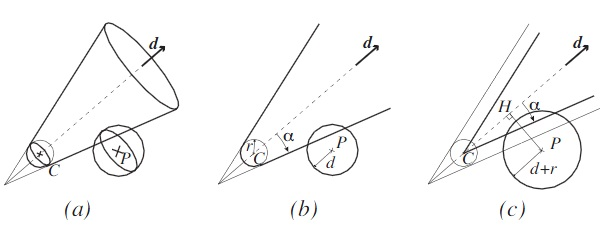
\includegraphics[scale=0.50]{Images/Node_Sphere_Intersection}
    \caption{\label{fig:crud2}Cone-Ray Union - 2D View. \small courtesy of \cite{Roger07}.}
\end{figure}

To calculate the intersection between the node, which is composed of the union of a sphere and a cone, we simplify the problem by enlarging the triangles bounding sphere \cite{Ericson04} and reducing the cones size (see Figure~\ref{fig:crud2}). The original formula for cone-sphere intersections was described in the Amanatides paper \cite{Amanatides84}. The current formula, which expands on the work of Amanatides, was described by Roger et al. \cite{Roger07}.

\begin{equation}
result = {|C - H|} \times \tan{\alpha} + \frac{d+r}{\cos{\alpha}} \geqslant
         {|P - H|}
\end{equation}

\subsection{Final Intersection Tests}

After traversing the hierarchy we have an array of node id and triangle id pairs. The candidates for the local intersection tests \cite{Moller97}. In this final step all that remains is to find out which is the closest intersected triangle for each ray and accumulate shading. Depending on the depth that we want for the algorithm we might need to output another set of secondary rays. Since the algorithm is generic, all that is necessary for this is to output these rays onto the ray array that we used initially and continue from the ray-sorting step.
